% Generated by code/ch01_measurement.py -- do not edit by hand.
\definecolor{qocA}{rgb}{0.00,0.45,0.70}
\definecolor{qocB}{rgb}{0.90,0.60,0.00}
\definecolor{qocC}{rgb}{0.00,0.62,0.45}
\definecolor{qocD}{rgb}{0.80,0.40,0.00}
\definecolor{qocE}{rgb}{0.80,0.60,0.70}
\definecolor{qocF}{rgb}{0.35,0.70,0.90}
\begin{tikzpicture}[]
\draw[thick] (0,0) circle (1.600);
\draw[dashed] (0,0) ellipse (1.600 and 0.560);
\draw[->] (0,0) -- (0,2.000) node[above] {$\ket{0}$};
\draw[->] (0,0) -- (0,-2.000) node[below] {$\ket{1}$};
\draw[->] (0,0) -- (1.800,0.000) node[right] {$x$};
\draw[->] (0,0) -- (-0.900,-0.400) node[above left] {$y$};
\fill (-0.194,-1.187) circle (1.5pt) node[above right, font=\small] {$\ket\psi$};
\draw[very thick, qocA, ->] (0,0) -- (-0.194,-1.187);
\begin{scope}[shift={(4.2,-1.8)}]
\begin{axis}[width=5.2cm, height=4.2cm, ybar, bar width=9pt, ymin=0, ymax=1, ylabel={$\Prob(0)$}, xtick=data,
  symbolic x coords={Born, $N{=}10$, $N{=}100$, $N{=}1000$}, tick label style={font=\scriptsize}, label style={font=\small},
  nodes near coords, nodes near coords style={font=\tiny}, enlarge x limits=0.18, xticklabel style={rotate=25, anchor=north east}]
\addplot[fill=qocA!60, draw=qocA] coordinates {(Born,0.206) ($N{=}10$,0.200) ($N{=}100$,0.230) ($N{=}1000$,0.199)};
\end{axis}
\end{scope}
\node[font=\small, align=center] at (6.6,2.1) {measure $\sigma_z$: outcome $0$ w.p. $\tfrac{1+r_z}{2}$,\\ then the state is destroyed};
\end{tikzpicture}
